\documentclass[
11pt, % The default document font size, options: 10pt, 11pt, 12pt
%oneside, % Two side (alternating margins) for binding by default, uncomment to switch to one side
english, % ngerman for German
singlespacing, % Single line spacing, alternatives: onehalfspacing or doublespacing
%draft, % Uncomment to enable draft mode (no pictures, no links, overfull hboxes indicated)
%nolistspacing, % If the document is onehalfspacing or doublespacing, uncomment this to set spacing in lists to single
%liststotoc, % Uncomment to add the list of figures/tables/etc to the table of contents
%toctotoc, % Uncomment to add the main table of contents to the table of contents
%parskip, % Uncomment to add space between paragraphs
%nohyperref, % Uncomment to not load the hyperref package
headsepline, % Uncomment to get a line under the header
%chapterinoneline, % Uncomment to place the chapter title next to the number on one line
%consistentlayout, % Uncomment to change the layout of the declaration, abstract and acknowledgements pages to match the default layout
]{MastersDoctoralThesis} % The class file specifying the document structure
% \usepackage[ngerman]{babel}
\usepackage{listings}
\usepackage{xcolor}

\definecolor{codegreen}{rgb}{0,0.6,0}
\definecolor{codegray}{rgb}{0.5,0.5,0.5}
\definecolor{codeorange}{rgb}{1,0.49,0}
\definecolor{backcolour}{rgb}{0.95,0.95,0.96}

\lstdefinelanguage{CSharp}{
    language=C,
    morekeywords={
        abstract, as, base, bool, break, byte, case, catch, char, checked, class, const,
        continue, decimal, default, delegate, do, double, else, enum, event, explicit, extern,
        false, finally, fixed, float, for, foreach, goto, if, implicit, in, int, interface,
        internal, is, lock, long, namespace, new, null, object, operator, out, override, params,
        private, protected, public, readonly, ref, return, sbyte, sealed, short, sizeof, stackalloc,
        static, string, struct, switch, this, throw, true, try, typeof, uint, ulong, unchecked,
        unsafe, ushort, using, virtual, void, volatile, while, var, dynamic, get, set
    },
    morecomment=[l]{//},
    morecomment=[s]{/*}{*/},
    morestring=[b]",
    sensitive=true
}

\lstdefinestyle{csharpStyle}{
    language=CSharp,
    backgroundcolor=\color{backcolour},   
    commentstyle=\color{codegray},
    keywordstyle=\color{codeorange}\bfseries,
    numberstyle=\tiny\color{codegray},
    stringstyle=\color{codegreen},
    basicstyle=\ttfamily\footnotesize,
    breaklines=true,                 
    captionpos=b,                    
    keepspaces=true,                 
    numbers=left,                    
    numbersep=10pt,                  
    showspaces=false,                
    showstringspaces=false,
    showtabs=false,                  
    tabsize=2,
    xleftmargin=1.5em,
    frame=none
}

\usepackage[utf8]{inputenc}
\usepackage[T1]{fontenc}
\usepackage{listings}
\usepackage{xcolor}
%\usepackage{fancyhdr} 
\usepackage[colorlinks=true, linkcolor=blue, citecolor=, urlcolor=red]{hyperref} 
\usepackage{float}
\usepackage{parskip}
\usepackage[style=numeric-comp, sorting=none, backend=biber]{biblatex} 
\addbibresource{literatur/literatur.bib}
\usepackage{tabularx}
\usepackage{array}
\renewcommand{\arraystretch}{1.2} 
\newcolumntype{Y}{>{\raggedright\arraybackslash\hspace{0pt}}X} 

\thesistitle{Netcode in Unity} % Your thesis title, this is used in the title and abstract, print it elsewhere with \ttitle

\supervisor{Prof. Dr. \textsc{Müller }} % Your supervisor's name, this is used in the title page, print it elsewhere with \supname

\examiner{Müller} % Your examiner's name, this is not currently used anywhere in the template, print it elsewhere with \examname

\degree{Bachelor of Business Information Systems} % Your degree name, this is used in the title page and abstract, print it elsewhere with \degreename

\author{Alexander \textsc{Seitz}} % Your name, this is used in the title page and abstract, print it elsewhere with \authorname

\addresses{} % Your address, this is not currently used anywhere in the template, print it elsewhere with \addressname

\subject{Business Information Systems} % Your subject area, this is not currently used anywhere in the template, print it elsewhere with \subjectname

\keywords{} % Keywords for your thesis, this is not currently used anywhere in the template, print it elsewhere with \keywordnames

\university{\href{http://www.h-ka.de}{Hochschule Karlsruhe}} % Your university's name and URL, this is used in the title page and abstract, print it elsewhere with \univname
\department{\href{http://department.university.com}{Business Information Systems}} % Your department's name and URL, this is used in the title page and abstract, print it elsewhere with \deptname

\group{\href{http://researchgroup.university.com}{Research Group Name}} % Your research group's name and URL, this is used in the title page, print it elsewhere with \groupname

\faculty{\href{http://faculty.university.com}{Wirtschaftsinformatik}} % Your faculty's name and URL, this is used in the title page and abstract, print it elsewhere with \facname

\AtBeginDocument{
\hypersetup{pdftitle=\ttitle} % Set the PDF's title to your title
\hypersetup{pdfauthor=\authorname} % Set the PDF's author to your name
\hypersetup{pdfkeywords=\keywordnames} % Set the PDF's keywords to your keywords
}

\usepackage{tikz}

\usepackage{tgheros}
\renewcommand*\familydefault{\sfdefault}


\begin{document}


\frontmatter % Use roman page numbering style (i, ii, iii, iv...) for the pre-content pages

\pagestyle{plain} % Default to the plain heading style until the thesis style is called for the body content

%----------------------------------------------------------------------------------------
%	TITLE PAGE
%----------------------------------------------------------------------------------------

\begin{titlepage}






\begin{figure}
\centering

\begin{tikzpicture}
		\node at (-1,13) { 
\includegraphics[width=5.652cm,height=1.507cm]{figures/logo.jpg} };
		\node at (-1,11) {Hochschule Karlsruhe};
		\node at (-1,10.5) {University of Applied Science};

		\node at (-1,9.5) {Fakultät für Informatik und Wirtschaftsinformatik};
		\node at (-1,9.0) {Wirtschaftsinformatik};
		\node at (-1,6.5) {BACHELORTHESIS};
		\node at (-1,5.0) {Netcode in Unity};

		  

\node at (-0.5,-2) { \begin{tabular}{p{3cm}p{10cm}}
Von		&			Alexander Seitz \\
&\\
Matrikelnr.	&		77642 \\
&\\
Arbeitsplatz		&	Hochschule Karlsruhe \\
&\\
Erstbetreuer		& Prof. Dr. Udo Müller \\
&\\
		  Zweitbetreuer	&	Prof. Dr. Jan Stöß \\
&\\
Abgabetermin	&	31.08.2025 \\

\end{tabular} };



\node at (3,-9.5) {\begin{tabular}{r}
Karslruhe, DATUM\\
\\
\\
Vorsitzender des Prüfungsausschusses
\end{tabular}
};

\end{tikzpicture}

\end{figure}


\end{titlepage}

\maketitle


\tableofcontents


\mainmatter
\chapter{Einleitung}
\label{chapter_1}
\newcommand{\keyword}[1]{\textbf{#1}}
\newcommand{\tabhead}[1]{\textbf{#1}}
\newcommand{\code}[1]{\texttt{#1}}
\newcommand{\file}[1]{\texttt{\bfseries#1}}
\newcommand{\option}[1]{\texttt{\itshape#1}}

Moderne Echtzeitanwendungen, insbesondere im Bereich der Computerspiele, stellen hohe Anforderungen an die zugrunde liegende Netzwerkarchitektur. Die Synchronisation von Spielzuständen, die Minimierung von Latenzzeiten sowie ein robuster Umgang mit Paketverlust und Jitter sind entscheidend für eine positive Nutzererfahrung. Multiplayer-Systeme, wie sie etwa mit Unity entwickelt werden, müssen deshalb nicht nur funktional, sondern auch leistungsfähig und fehlertolerant sein.

Die vorliegende Arbeit beschäftigt sich mit den theoretischen und technischen Grundlagen der Netzwerkkommunikation in Mehrspielerumgebungen. Anhand eines prototypischen Projekts in Unity werden exemplarisch zentrale Mechanismen wie Reconciliation, Interpolation sowie die Kommunikation im Client-Server-Modell umgesetzt und analysiert.

Im Folgenden werden zunächst die Motivation und Zielsetzung der Arbeit erläutert. Anschließend wird der strukturelle Aufbau der Arbeit vorgestellt.

\section{Motivation}
In den meisten modernen Spielen ist oft ein Teil des Spiels als Mehrspieler ein kooperativer Teil des Spiels integriert. Diese Bereiche reichen von strategischen FPS, Survival-Spielen bis zu Rennspielen. In all diesen Spielen wird von den Spielern ein hoher Wert auf Genauigkeit und Funktionalität des Netcode-Systems verlangt.
Diese Integration bringt oft sehr viele Herausforderungen, in manchen Fällen ist auch eine komplette Eigenimplementierung auf Grund der Komplexität von der Basis des Spiels nicht abzudenken. Viele Entwickler vor allem Indie-Entwickler, stellen wenn überhaupt einen Mehrspieler erst einmal hinten an, da eine ausgereifte Integration vor allem für Unerfahrene eine große Herausforderung werden kann. 

Im Bereich der AAA-Titel jedoch, kommt es immer häufiger zu Kritikäußerungen von Medien als auch Spielern. In vielen Fällen wird sich auf die kostensparenden Ansätze der Entwickler beziehungsweise der Publisher der Spiele bezogen, die sich für billigere und somit leistungsärmere Alternativen wie bspw. Server mit niedrigeren Tickraten entscheiden.
In den letzten Jahren kam jedoch eine der kuriosesten Neuerungen in den Mainstream der strategischen FPS, nämlich sollte das Counter Strike 2 -- der direkte Nachfolger von CS:GO -- auf Grundlage eines Subtick-Systems implementiert werden, anstatt das altbewährte klassische Ticksystem zu verbessern und modernisieren.
Das System existierte schon vor der Integration des beliebten FPS, dennoch wurde es nie konsequent oder erfolgreich integriert. 
Subtick ist im Grunde ein eigenes Ticksystem zwischen Ticks, demnach ist jeder Input mit einem konkreten Timestamp versehen und soll rein theoretisch, zu genaueren und direkterem Spielgefühl führen.
Beim Klassischen System werden Eingaben zwischen Ticks an den nächsten Tick delegiert, was Synchronisation zwischen Clients oft erschwert bzw. oft zu uneinheitlichen Erfahrungen fürht.

Demnach liegt die Frage nahe, ob es sich wirklich um ein Problem beim Entwickler handelt oder ein Problem, von maßloser Komplexität, die von so vielen Variablen abhängt, dass sie in keinem Fall zu perfektionieren ist.
(Das könnte man auf jeden Fall ändern, war nur das erste was mir eingefallen ist).
\section{Zielsetzung}
In dieser Arbeit sollen Netcode und darauf aufbauende Netcode Mechanismen auf theoretischer und praktischer Grundlage beleuchtet werden und in einem prototypischen Spiel integriert werden.
Da die reine Umsetzung keinen großen akademischen Mehrwert bietet, sollen Strategien entworfen werden, die zur Visualisierung und damit hoffentlich der Verbesserung des Verständnisses der Mechaniken dienen.
Es sollen des weiteren verschiedene Szenarien untersucht werden, die auch von Idealbedingungen abweichen können.
\chapter{Auswahl der Engine}
Um die bestmöglichste und vor allem effizienteste Entwicklung des Spiels und der geplanten Netcode Mechanismen zu integrieren, ist also eine durchdachte Wahl der Spiel Engine wichtig.
Da vor allem Zeit ein Engpass in einem ambitionierten Projekt, wäre es fatal, wenn auf Grund der Wahl der Engine kein Fortschritt gemacht werden kann. 
Die wichtigsten Kriterien werden im Folgenden aufgelistet.

\section{Lernkurve}
Eine der wichtigeren Aspekte bezieht sich auf die Lernkurve der Game Engine für den Entwickler. Wenn also eine Engine mit so viel Lernaufwand in Verbindung steht um überhaupt eine triviale Szene zum Laufen zu bekommen, dann ist diese wohlmöglich nicht die richtige Engine.
Im Anbetracht dieser Arbeit ist Zeit die wichtigste Ressource und darf somit nicht unterschätzt werden. Wenn somit Zeit gespart werden kann, indem man eine einsteigerfreundliche Engine lernen kann, ist das für die anstehende Entwicklungsarbeit ein Erfolg~. 
Wenn jedoch gewisse Vorkenntnisse im Bereich Spieleentwicklung bestehen sollten, dann wird das Erlernen einer weiteren Engine, was mit viel duplikativem Wissen im Zusammenspiel steht, für wesentlich geringern Lernaufwand sorgen. Unter dieser Bedingun ist der Lernaufwand wiederum keine   

\section{Community und Ressourcen} 
Die Zugänglichkeit von Dokumentation, Foren und Tutorials ist in diesem Kontext extrem wertvoll, da vor allem die Kombination daraus ein tiefes Verständnis einbringen kann. Wenn also die Dokumentation nicht verständlich sein sollte oder es nicht genug Anwendungsbeispiele im Internet geben sollte, kann es den Lernaufwand zusätzlich erhöhen oder zu Missverständnissen kommen.

\section{Netcode-Fähigkeiten}
Wenn also "out of the box" Features gut integriert und dokumentiert sind, die die Weiterentwicklung geplanter Netcode-Mechaniken erleichtern, ist dies der Idealzustand. 
Dennoch ist für diese Arbeit eine Abgrenzung zu machen, da die Eigenimplementierung im Mittelpunkt steht. Wenn also Mechanismen von der Engine bereits zum Großteil gestellt sind und der Quellcode hiervon nicht anpassbar ist, wirkt sich dies eher negativ auf die Bewertung aus.

\section{Performance}
Wie gut das Spiel im Einsatz von mehreren Clients läuft und wie viele Einbuße in diesem Fall der Multiplayer-Aspekt mit sich bringt. Sollte dies jedoch garnicht mehr möglich sein, dass ein Editor und ein oder mehrere Clients verbunden sind - was im Grunde das Laufen von drei Spielinstanzen darstellt - nicht funktionieren sollte, weil keine Ressourcen mehr auf dem Computer übrig bleiben, ist dies wohl keine geeignete Engine oder man muss optimieren. 
Allerdings kann eine graphische Grundvoraussetzung zum Problem werden. Wenn also die Engine durch die Natur der Renderpipeline zu sehr die GPU belastet, kann das schon das Prototyping beeinflussen, da in diesem Use Case eine hohe Framerate bevorzug ist.

\section{Kosten und Lizenzmodell}
Viele der bekannten Engines sind nicht Open Source sondern erwarten i.d.R. eine jährliche Zahlung oder eine Art Pacht~. In manchen Fällen ist eine jährliche Hochschullizenz möglich, dennoch fällt das somit immernoch unter die Kategrie der Zahlungspflicht. 
Wenn eine Engine somit einen hohen monetären Einsatz erfordert ohne der Möglichkeit auch nur auf eine bspw. Testversion zuzugreifen, müssen die anderen Aspekte sehr viel gutmachen.

\section{Programmiersprache}
In vielen Fällen steht für den Entwickler ein hoher Lernaufwand mit einer noch zu erlernenden Programmiersprache, bei der neue Aspekte in den Mittelpunkt gerückt werden, die u.U. noch nicht zuvor behandelt wurden. In den meisten Fällen sind dies eher hardwarenähere Programmiersprachen wie bspw. C++. Hierbei müssen neue Konzepte wie der Umgang mit Memory erlernt und gemeistert werden, was im Umgang mit neueren Programmiersprachen wie C\# schon bereits gestellt ist. 
Im Grunde stellt das nicht nur ein Risiko dar, sondern ist auf der anderen Seite auch eine Chance zu lernen, wie man richtig Spiele entwickelt und vor allem auch Quellcode optimieren kann. Nicht ohne Grund bauen die meisten Spiele-Engines auf C++ auf und werden in der Zukunft auch eher nicht ersetzt.  

\section{Marktrelevanz}
Die Marktrelevanz ist wie in {Programmiersprache} schon angesprochen, stark abhängig von der in der Engine genutzten Programmiersprache. Abgesehen davon gibt es unterschiedliche Einsatzbereiche verschiedener Engines und somit lässt sich die Marktrelevanz nicht nach absoluten Zahlen der Nutzter und oder bestimmter Spiele klären. Dennoch muss man die Relevanz der Engine im Auge behalten, wenn es also kaum Spiele auf dem Markt gibt, die mit einer bestimmten Engine entwickelt wurden, dann ist die potenziell investierte Zeit in einer beliebteren Engine wahrscheinlich angebrachter.


%\begin{itemize}
    %\item \textbf{Lernkurve}: Wie zugänglich ist die Engine für Entwickler mit unterschiedlichen Erfahrungsstufen? 
    %\item \textbf{Community und Ressourcen}: Verfügbarkeit von Dokumentationen, Tutorials und aktiver Community.
    %\item \textbf{Netcode-Fähigkeiten}: Wie gut lässt sich Multiplayer-Logik implementieren? 
    %\item \textbf{Performance}: Optimierungsmöglichkeiten für verschiedene Plattformen, insbesondere im Multiplayer-Bereich.
    %\item \textbf{Kosten und Lizenzmodell}: Wie gut zugänglich sind die einzelnen Produkte?
    %\item \textbf{Programmiersprache}: Wie viel Zusatzaufwand fällt für den Entwickler zu seiner aktuellen Situation zusätzlich noch an? In einem Fall, dass eine hardwarenähere Sprache erlernt oder vertieft werden muss. Ein Beispiel wäre hierbei UE5 und C++: Es muss hierbei sehr viel an low level coding erlernt werden... 
    %\item \textbf{Marktrelevanz}: Wie etabliert ist die Engine in der Spielebranche? 
%\end{itemize}

\newpage

Ein direkter Vergleich der bekanntesten Engines zeigt folgende Eigenschaften:

\begin{table}[H]
\centering
\caption{Vergleich populärer Spiel-Engines mit Gewichtung}
{\small
\begin{tabularx}{\textwidth}{|l|c|Y|Y|Y|}
\hline
\textbf{Kriterium} & \textbf{Gewichtung} & \textbf{Unity} & \textbf{Unreal Engine} & \textbf{Godot} \\
\hline
Programmiersprache & 3 & C\# & C++ / Blueprints & GDScript / C\# \\
\hline
Lernkurve & 5 & Mittel & Hoch & Niedrig \\
\hline
Community & 4 & Sehr groß & Groß & Wächst schnell \\
\hline
Netcode & 5 & NGO, FishNet u.a. & Eigenes Replication-System & Drittanbieter, rudimentär \\
\hline
Performance & 4 & Gut (abhängig von Optimierung) & Sehr hoch & Mittel \\
\hline
Lizenz / Kosten & 5 & Kostenlos (eingeschränkt), Runtime Fee seit 2024 \cite{unitylicense} & Royalty-basiert \cite{unrealpricing} & Open Source \cite{godotdoc} \\
\hline
Verbreitung in Industrie & 3 & Sehr hoch & Hoch & Gering \\
\hline
\textbf{Gesamtbewertung} & – & \textbf{–} & \textbf{–} & \textbf{–} \\
\hline
\end{tabularx}
}
\end{table}

Die Quantifizierung wurde auf Grundlage einer Skala von 1-5 bewerkstelligt, wobei 5 das Maximum ist und somit am besten. Diese Werte dienen als Multiplikatoren mit den Werten (ebenfalls 1-5) der einzelnen Spalten. Beide Skalen sind subjektiv und sind somit auch stark von Vorkenntnissen abhängig. 
Die einzelnen Spalten jedoch sind keine Gewichtungen sondern eher die tatsächlichen Werte, die vergeben wurden. 


\newpage
Basierend auf den genannten Faktoren fiel die Wahl auf \textbf{Unity}, da diese Engine eine ausgewogene Kombination aus Zugänglichkeit, Flexibilität und Netcode-Erweiterbarkeit bietet. \\
Besonders die Integration von C\# als Programmiersprache, die umfangreiche Dokumentation sowie die breite Community-Unterstützung waren ausschlaggebend. Demnach ist Unity vor allem auch am einsteigerfreundlichsten, was im Endeffekt Komplexität reduziert.

Unreal Engine hingegen spielt vor allem in der Entwicklung moderner, grafisch anspruchsvoller Spiele eine zentrale Rolle. Während Unity und Godot insbesondere im Indie-Bereich weit verbreitet sind, wird Unreal Engine regelmäßig für sogenannte AAA-Titel eingesetzt -- etwa bei \textit{Fortnite}, \textit{Valorant} oder der \textit{Gears of War}-Reihe. In Addition kommt noch eines der am meist antizipiertesten Spiele überhaupt dazu nämlich The Witcher 4 \cite{witcher-4-demo}. 

Ein besonderes Beispiel für die Weiterentwicklung der Engine durch Eigengebrauch ist das Prinzip des „Dogfooding“. Epic Games nutzt die Unreal Engine intern intensiv zur Entwicklung eigener Spiele wie \textit{Fortnite}, wodurch neue Features -- etwa das Partikelsystem \textit{Niagara} -- direkt unter realen Produktionsbedingungen erprobt und optimiert werden \cite{dogfoodingexample}.

Insbesondere mit der Einführung von Unreal Engine 5 (UE5) hat sich die Engine als Standardlösung für kleinere bis mittlere Studios etabliert, die auf fotorealistische Darstellung und moderne Grafiktechnologien wie \textit{Lumen} oder \textit{Path Tracing} setzen. Unity kann in diesen Bereichen zwar nicht vollständig mithalten, bietet jedoch im Kontext dieser Arbeit -- etwa bei der prototypischen Umsetzung netzwerkbasierter Mechaniken -- eine effizientere und zugänglichere Plattform. Beispiele wie \textit{BattleBit Remastered} (2023) jedoch zeigen, dass auch technisch reduzierte, aber netzwerkseitig ausgereifte Multiplayer-Titel mit Unity erfolgreich realisiert werden können.

\section{Eigenimplementierung und Auswahl des Frameworks}

Im Bereich Netcode existieren für Unity verschiedene Frameworks. Zunächst wurde Unitys offizielles \textbf{Netcode for GameObjects (NGO)} in Betracht gezogen. NGO ist mit Netcode for Entities der Standard und das als eigenes Paket, welches man über den Package Manager installieren kann.   In der praktischen Erprobung zeigten sich jedoch Schwächen im zugrunde liegenden \textit{Tickmodell}. NGO nutzt ein festes Zeitraster zur Synchronisation zwischen Server und Clients, wobei alle Netzwerkaktionen strikt an die sogenannte \textit{NetworkTick}-Rate gebunden sind.

Dieses Modell ist zwar grundsätzlich stabil, führt jedoch bei Spielen mit hoher Eingabefrequenz oder schnellen Bewegungsabläufen zu Einschränkungen: Eingaben, die zwischen zwei Ticks liegen, werden verzögert verarbeitet, was sich in Form von spürbarer Latenz oder schwankender Reaktionsgeschwindigkeit äußern kann. Besonders bei deterministisch kritischen Anwendungen erschwert dies eine präzise Umsetzung von Mechaniken wie Client-Side Prediction oder Server Reconciliation. 
Hierfür müsste ein Ticksystem selbst implementiert werden, was je nach Architektur zu Kollisionen führen kann.

Als Alternative wurde das Framework \textbf{FishNet} in Betracht gezogen, das in der offiziellen Dokumentation ausdrücklich für Anwendungsfälle mit hohen Anforderungen an Präzision und deterministische Logik empfohlen wird \cite{fishnetdocs}. FishNet nutzt ein eigenes Tick-basiertes Netzwerkmodell und bietet unter anderem:

\begin{itemize}
    \item Vollständige Kontrolle über Netzwerklogik
    \item Support für Host-Modus, Dedicated Server und Peer-to-Peer
    \item Integration mit Prediction, Interpolation und Authentifizierung
\end{itemize}

Trotz dieser technischen Vorteile wurde für diese Arbeit letztlich \textbf{NGO verwendet}. Hauptgrund war zum einen der geringere Integrationsaufwand und die direkte Unterstützung durch Unity. Eine vollständige Migration auf FishNet hätte umfangreiche Anpassungen erfordert, die im gegebenen Zeitrahmen nicht realisierbar gewesen wären.
Fishnet nutzt somit oft auch eine andere Syntax, die nicht so weit verbreitet ist wie der Standard von Unity's NGO. Dies macht die Fehlerbehebung komplizierter und führt vor allem bei Netcode-Unerfahrenen zu Komplikationen.  
In der Dokumentation ist ebenfalls nichts zur Portierung von NGO auf Fishnet enthalten, was die Umstellung deutlich aufwändiger und zeitlich bedingt riskanter machen würde. Hierfür wäre sogar ein kompletter Umbau nötig und selbst damit könnte Erfolg nicht garantiert sein. 
Abgesehen davon, ist Fishnet sehr reich an Features, die über die Mindestanforderungen hinausgehen. In jedem anderen Use Case wäre Fishnet wohl die beste Entscheidung, weil es die sinnvollste und beste Vorablösung bereitstellt, dessen Umbau jedoch in keinster Weise trivial ist.

Zum anderen liegt der Schwerpunkt dieser Arbeit explizit auf dem \textbf{Verständnis und der eigenständigen Implementierung} zentraler Netcode-Mechaniken wie \textit{Client-Side Prediction}, \textit{Server Reconciliation} und \textit{Interpolation}. Statt auf bereits vollständig implementierte Framework-Funktionalitäten zurückzugreifen, wird ein eigenes, leichtgewichtiges System entwickelt, um die Funktionsweise dieser Konzepte praktisch und nachvollziehbar umzusetzen.

NGO wird hierbei vor allem als \textit{Basisschicht} für die Netzwerkkommunikation genutzt, während zentrale Mechanismen unabhängig davon realisiert werden. Dieser Ansatz erlaubt eine tiefere Auseinandersetzung mit den zugrunde liegenden Prinzipien und Herausforderungen im Netcode-Design.

\chapter{Beschreibung des Unity Prototyps}

Der entwickelte Prototyp  bildet eine einfache First-Person-Shooter-Sandbox ab und dient als Testumgebung für die Untersuchung netzwerkbezogener Mechaniken wie Interpolation, Client-Side Prediction und Lag Compensation. Der Prototyp wird auch zum Abschluss der Arbeit bewusst schlicht gehalten, da der Fokus auf der Netzwerkschicht liegt – nicht auf grafischen oder animationsbasierten Aspekten. Texturen, Beleuchtung und Animationen wurden daher nur in minimalem Umfang berücksichtigt.
Im Verlauf der Arbeit existieren prinzipiell zwei Versionen, bei denen es sich zum einen um die Grundstruktur des Spiels gekümmert werden musste, was demnach den Offline-Prototypen darstellt. Diese Version besteht aus fundamentalen aber auch sehr schlicht gehaltenen Bestandteilen für ein FPS-Spiel. Diese bestehen aus einem Character Controller mit dem man springen und laufen kann und einer Waffe in First-Person-Ansicht, die über eine Schuss- und Nachlademechanik verfügt. 
Ein Schadensmodell, das als Metadaten den einzelnen Waffen zugewiesen werden kann und das alles auf einer minimalistischen Prototyp-Map.
Auf diesem Prototypen anknüpfend, sollen und wurden besagte Netcode-Mechaniken inklusive Synchronisation integriert werden.   

\newpage
\section{Szenario und Spiellogik}
Die Umgebung erinnert an Aim-Trainingsszenarien aus Spielen wie \textit{Valorant} (Range) oder eigenständigen Tools wie \textit{Aim Lab}. Der Spieler wird durch einen FPS-Controller dargestellt, der als \texttt{Prefab} implementiert ist. In der Szene bewegen sich ein oder mehrere Zielobjekte (Targets), die sich zufällig und unvorhersehbar über das Spielfeld bewegen. Diese Targets können wiederholt erscheinen (respawnable) und dienen im späteren Verlauf zur Untersuchung netzwerkbedingter Bewegungsartefakte.
Zusätzlich können sich mehrere Clients auf den Server verbinden und sollen synchronisiert werden. Hierbei geht es darum Inputlatenz auch bei hohem Ping minimal zu halten und ein flüssiges und direktes Spielgefühl zu erlauben auch bei hoher Latenz.


\section{Waffenmechanik und Spielgefühl}
Für das Waffenmodell wurde ein Asset aus dem Unity Asset Store verwendet\footnote{Platzhalter: \textit{Name des Assets einfügen}}, da die Eigenmodellierung in Blender aus zeitlichen Gründen verworfen wurde. Dennoch wurden grundlegende FPS-typische Elemente integriert:

\begin{itemize}
  \item Rückstoß (Recoil)
  \item Bewegungsbasiertes Waffenbobbing und Sway
  \item Mündungsfeuer (Muzzle Flash)
  \item Einschusslöcher (Decals)
\end{itemize}

Diese Features verbessern nicht nur das Spielgefühl, sondern sind auch eine wichtige Grundlage für die spätere visuelle Analyse der Netzwerkmechaniken. Die Netzwerksynchronisation solcher Effekte gilt als nicht trivial und ist auch in professionellen Produktionen fehleranfällig und wird demnach ebenfalls ausgelassen.
Spielerobjekte werden in Unity meistens über ein eigenes Network-Transform synchronisiert, welches in der Regel hauptsächlich nur Für die Position des jeweiligen Transforms zuständig ist. Wenn also Einschusslöcher synchronisiert werden müssen oder Animationen bzgl. der Waffen muss dies auf anderer Ebene entstehen was auch zu Kollisionen mit dem bereits verwendetem Network Transform. 

\section{Technische Herausforderung: Raycasting}
Ein zentrales technisches Problem ergab sich bei der Definition des Ursprungs der Schusslinie (Raycast). Zwei gängige Ansätze wurden gegenübergestellt:

\begin{enumerate}
  \item Raycast vom Lauf der Waffe (Mündung)
  \item Raycast aus dem Zentrum der Kamera (Fadenkreuz)
\end{enumerate}

Für den Prototyp wurde Variante 2 gewählt, da diese Methode eine konsistentere Treffergenauigkeit gewährleistet und im Hinblick auf Debugging und Netzwerkanalyse einfacher zu handhaben ist.

\section{Netzwerkarchitektur des Prototypen}
Der Prototyp basiert auf dem \textit{Netcode for GameObjects}-Framework von Unity und nutzt ein Server-Client-Modell. Clients werden über den Unity-Build gestartet und mit einem lokalen Server verbunden. Netzwerkkomponenten wie Zustandsübertragung und Objektregistrierung erfolgen aktuell noch über Unitys \texttt{NetworkTransform}-Komponente.

Diese Komponente erlaubt eine schnelle Prototypenerstellung, übernimmt jedoch automatisch Funktionen wie Interpolation und Zustandssynchronisation. Für die Zwecke dieser Arbeit ist dies ungeeignet, da keine gezielte Kontrolle oder Analyse der einzelnen Netzwerkmechanismen möglich ist. 

\subsection{Ausblick:}
In den kommenden Entwicklungsschritten soll die \\ \texttt{NetworkTransform}-Komponente teilweise durch eine eigene Implementierung ersetzt werden, um die Funktionsweise und Auswirkungen von Interpolation, Prediction, Reconciliation und Lag Compensation explizit untersuchen und visualisieren zu können.

\chapter{Analysewerkzeuge für Netcode und Debugging}

Zur Untersuchung netzwerkbasierter Spielmechaniken wie Client-Side Prediction, Lag Compensation oder Interpolation ist der Einsatz geeigneter Analysewerkzeuge essenziell. Ziel ist es, sowohl das Verhalten dieser Mechaniken unter verschiedenen Bedingungen zu verstehen, als auch deren Einfluss auf das Spielgefühl sichtbar und messbar zu machen.

Im Rahmen dieser Arbeit soll ein System verwendet werden, bestehend aus einem Debug-Overlay und einer integrierten Ingame-Konsole. Dieses Werkzeug ermöglicht es, netzwerkrelevante Parameter -- wie beispielsweise Interpolationszeiten, künstliche Latenz oder Glättungsalgorithmen -- zur Laufzeit zu verändern. Alternativ wird dies nach herkömmlichem Ablauf über Netzwerkvariablen im Unity-Editor  \\
So lassen sich spezifische Szenarien gezielt nachstellen und deren Auswirkungen visuell nachvollziehen.

Neben dieser Eigenentwicklung existieren auch externe Lösungen, wie etwa der Unity Profiler mit Netcode-Unterstützung oder Werkzeuge von Drittanbietern wie Photon Fusion Analyzer. Diese bieten detaillierte technische Einblicke, sind jedoch oft nicht für eine interaktive Analyse innerhalb des Spiels ausgelegt.

Für die Konsole, die auch in Spielen wie Counter Strike oder anderen Spielen existiert um ohne Benutzeroberfläche Einstellungen zu ändern, wird hier aus dem Unity Asset Store bezogen. \cite{}
Mit diesem Asset lassen sich Konsolen-Kommandos im Quellcode registrieren, die den Spielfluss manipulieren können. Außerdem ist auch das Auslesen der Debugging-Konsole möglich wenn man im Build ist, welcher keine integrierte Konsole besitzt wie der normale Editor.

Das entwickelte Debug-System hingegen erlaubt eine tiefere Integration in den Entwicklungsprozess: Es zeigt Zustände wie die aktuelle Netzwerkverzögerung, Tick-Synchronisation oder Prediction-Fehler direkt im Spiel an. Ergänzend dazu erlaubt die Konsole das Aktivieren und Deaktivieren einzelner Netcode-Komponenten oder das dynamische Nachjustieren von Parametern -- ohne das Spiel neu starten zu müssen.

Durch diese Flexibilität ist das System besonders geeignet für die iterative Entwicklung und Bewertung von Netcode-Strategien und stellt daher das zentrale Analysewerkzeug dieser Arbeit dar.



\chapter{Client-side Prediction \& Reconciliation}
Im folgenden Abschnitt werden die im Projekt umgesetzten und verwendeten Mechaniken beschrieben und anhand des Quellcode beschrieben.
Hierbei liegt der Fokus darauf, ein durchdachtes System zu verwenden, das den Kern der Problematik einfach im Spiel erkenntlich machen kann. 

\section{Client-side Prediction beim Bewegen und Schießen}

In einem serverautoritativen Netzwerkmodell ist es essenziell, ein faires und sicheres Spielumfeld zu gewährleisten. Gleichzeitig darf die Spielbarkeit aus Sicht des Spielers nicht unter einer hohen Latenz leiden. Besonders bei reaktionsintensiven Genres wie First-Person-Shootern oder Rennspielen ist eine direkte Rückmeldung auf Eingaben entscheidend für das Spielerlebnis.

Ein vollständiger Verzicht auf Client-Authorität würde zwar maximale Sicherheit bieten, jedoch zu spürbarer Verzögerung bei der Bewegung oder Aktion führen. Ziel ist daher ein Kompromiss: Der Server behält die Entscheidungsgewalt, während der Client Eingaben sofort lokal umsetzt und visuelles Feedback liefert.

\newpage
In der vorliegenden Implementierung wird dies durch ein Überschreiben der Unity-eigenen \texttt{NetworkTransform}-Komponente realisiert. Die Autoritätslogik wird über eine einfache Enumeration gesteuert:

\lstinputlisting[
  style=csharpStyle,
  caption={Überschreiben der NetworkTransform-Komponente mit AuthorityMode},
  label={lst:authority-mode} 
]{src/PlayerMovement/ClientNetworkTransform.cs}


Die Methode \texttt{OnIsServerAuthoritative()} gibt in der Regel \texttt{false} zurück, sodass der Client die Kontrolle über Bewegung und Eingabe erhält, ohne dass ein Roundtrip zum Server erforderlich ist. Dadurch wird die Latenzwahrnehmung beim Spieler erheblich reduziert.


\newpage
\section{Reconciliation – Zustandskorrektur  bei Abweichungen}

Trotz lokaler Vorhersage durch den Client bleibt der Server die Referenzinstanz für den „wahren“ Spielzustand. Sollte es zu größeren Abweichungen zwischen Client- und Serverposition kommen, wird ein Reconciliation-Prozess ausgelöst. Dabei wird der Client zurück auf den zuletzt vom Server bestätigten Zustand gesetzt und die eigenen Eingaben ab diesem Zeitpunkt erneut simuliert.

In Spielen mit präzisem Bewegungsfeedback (z.B. FPS) ist die Toleranzschwelle für Positionsfehler oft sehr gering. In diesem Projekt wurde ein Grenzwert: \\ (\texttt{reconciliationThreshold}) definiert, ab dem eine Zustandskorrektur erfolgt. Dieser Wert kann abhängig von variabler Netzwerklatenz angepasst werden.

\begin{figure}[H] % oder [htbp]
    \centering
    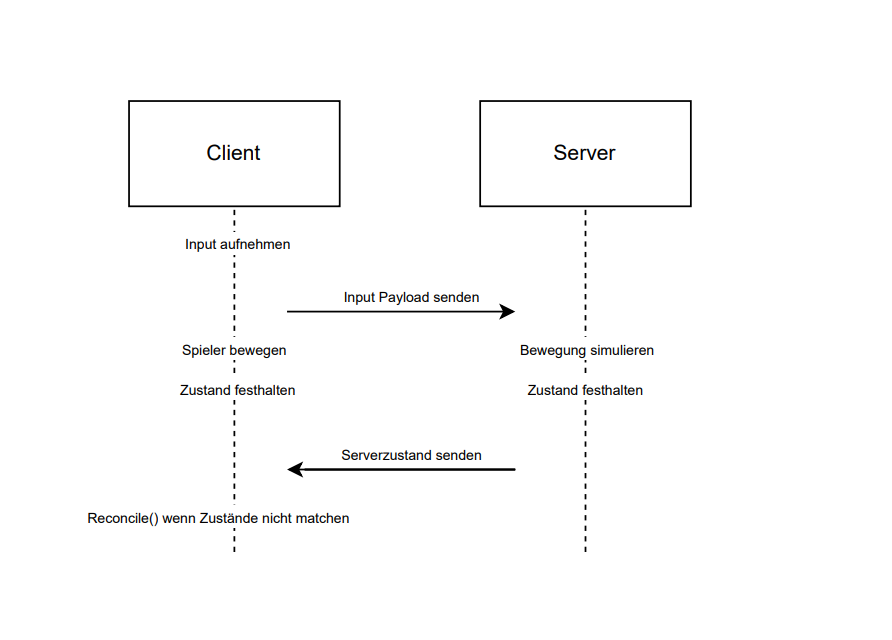
\includegraphics[width=0.8\textwidth]{figures/ReconciliationSeq.png}
    \caption{Sequenzdiagramm Reconciliation}
    \label{fig:logo}
\end{figure}

\section{Testmechanismus zur Validierung}

Zur gezielten Auslösung der Reconciliation wurde ein einfacher Testmechanismus implementiert: Ein Client-Cheat teleportiert den Spieler um 20 Einheiten nach vorne – weit über die Fehlertoleranz hinaus. Der Server erkennt die Abweichung und triggert die Korrektur, wodurch der Spieler sichtbar in den korrekten Zustand „zurückspringt“.

Zur Visualisierung wurden farblich unterschiedliche Proxies (3D-Würfel) über dem Spielerobjekt angezeigt, die die vom Client bzw. Server berechneten Zustände darstellen.

\section{Datenstrukturen und Ticksystem}
Als Datenstruktur wurde für das Ticksystem auf zirkuläre Buffer gesetzt. Im Netcode-Bereich ist dies defacto Standard <Quelle maybe> um die mit den einzelnen Ticks verbundenen Informationen oder genauer Positionen, Rotationen und Geschwindigkeiten umzugehen und Overheads zu negieren.
Demnach eignen sich bspw. Arrays oder Dictionaries deutlich schlechter, da diese die gespeicherten Informationen nicht verwerfen und somit unnöitge Daten halten, die für bspw. die Reconciliation außer Reichweite liegen und somit die Performance beeinträchtigen.
In Kombination mit State und Input Payloads die jeweils als Structs implementiert wurden, sollen die Positionen zum passenden Tick verglichen werden können.
Die Eigenimplementierung des Circular Buffer ist somit generisch und basiert auf den Input oder State Payloads. Mit der Methode Add(), die ein generisches Item also in diesem Fall das State oder Input Payload und einen Index als Parameter nimmt, kann somit der Buffer befüllt werden.
Das Befüllen folgt den algorithmischen Grundlagen eines solchen Buffers und das geschieht bis zu der statischen Buffergröße und fängt dann wieder von null an zu indezieren. 
Somit werden in diesem Fall intern also bis 1024 Ticks verwaltet, was bei einer Standard-Tickrate von 60Hz ungefähr 17 Sekunden wären, die man zurückspulen könnte.
Eine solche Buffergröße ist im Grunde schon relativ großzügig, sollte man jedoch auf eine Tickbasis aufsteigen von etwa 128Hz, ist es schon etwas sinnvoller.  (vielleicht noch erwähnen warum genau...) 

\newpage

Im Folgenden sieht man noch den Aufbau des Circular Buffers und die Strukturen die essentiell sind für den Datentransfer:
\lstinputlisting[
  style=csharpStyle,
  caption={Methode \texttt{CircularBuffer()}},
  label={lst:circular-buffer}
]{src/CircularBuffer.cs}

\newpage
Auf der anderen Seite muss dies durch die angesprochenen Strukturen gespeichert werden:
\lstinputlisting[
  style=csharpStyle,
  caption={Methode \texttt{Payload}},
  label={lst:payload}
]{src/Payload.cs}
In der InputPayload werden die Eingabedaten des Spielers verwaltet und serialisiert, was über die vom zu implementierenden Interface INetworkSerializeable gestellten Methode NetworkSerialize() getan wird.

\section{Kernmethoden der Reconciliation-Logik}
Im Grunde lässt sich die Logik auf einige Methoden runterbrechen, dies sich alle im PlayerMovement Skript befinden. Diese Methoden sind jedoch verschachtelt in einem komplexeren Ablauf dieses Skriptes, reichen aber fürs Verständnis aus. 
\newpage
\begin{enumerate}
    \item \texttt{ShouldReconcile()} \\
    Diese Methode prüft, ob neue Serverdaten vorliegen und ob diese sich vom zuletzt verarbeiteten Zustand unterscheiden:

\lstinputlisting[
  style=csharpStyle,
  caption={Methode \texttt{ShouldReconcile()}},
  label={lst:should-reconcile}
]{src/PlayerMovement/ShouldReconcile.cs}

    \item \texttt{ReconcileState(StatePayload rewindState)} \\
    Hier wird der Client-Zustand auf den vom Server bestätigten Zustand zurückgesetzt. Anschließend werden alle seitdem aufgezeichneten Eingaben erneut angewendet:

\lstinputlisting[
  style=csharpStyle,
  caption={Methode \texttt{ReconcileState(StatePayload)}},
  label={lst:reconcile-state}
]{src/PlayerMovement/ReconcileState.cs}

    \item \texttt{HandleServerReconciliation()} \\
    Diese Methode koordiniert den gesamten Reconciliation-Prozess und vergleicht die Zustände beider Seiten:

\lstinputlisting[
  style=csharpStyle,
  caption={Methode \texttt{HandleServerReconciliation()}},
  label={lst:handle-server-reconciliation}
]{src/PlayerMovement/HandleServerReconciliation.cs}
\end{enumerate}


\printbibliography

\end{document}
